\documentclass[a4paper]{article}
\setlength{\voffset}{0mm}
\setlength{\topmargin}{0mm}
\setlength{\headheight}{0mm}
\setlength{\headsep}{0mm}
\setlength{\textheight}{256mm}
\setlength{\hoffset}{0mm}
\setlength{\marginparwidth}{0mm}
\setlength{\evensidemargin}{0mm}
\setlength{\oddsidemargin}{0mm}
\setlength{\textwidth}{160mm}
\usepackage{graphicx}

\begin{document}

\title{Introduction to \LaTeX{}}
\author{Author's Name}

\maketitle

\begin{abstract}
The abstract text goes here.
\end{abstract}

\section{Introduction}
Here is the text of your introduction.

\begin{equation}
    \label{simple_equation}
    \alpha = \sqrt{ \beta }
\end{equation}

\subsection{Subsection Heading Here}
Write your subsection text here.

\begin{figure}
    \centering
    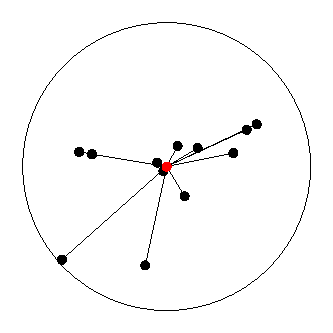
\includegraphics[width=3.0in]{fig-compactness.eps}
    \caption{Simulation Results}
    \label{simulationfigure}
\end{figure}

\section{Conclusion}
Write your conclusion here.

\end{document}

